\documentclass[tikz,border=3.14mm]{standalone}
\usepackage{pgfplots}
\pgfplotsset{compat=1.17}

\begin{document}
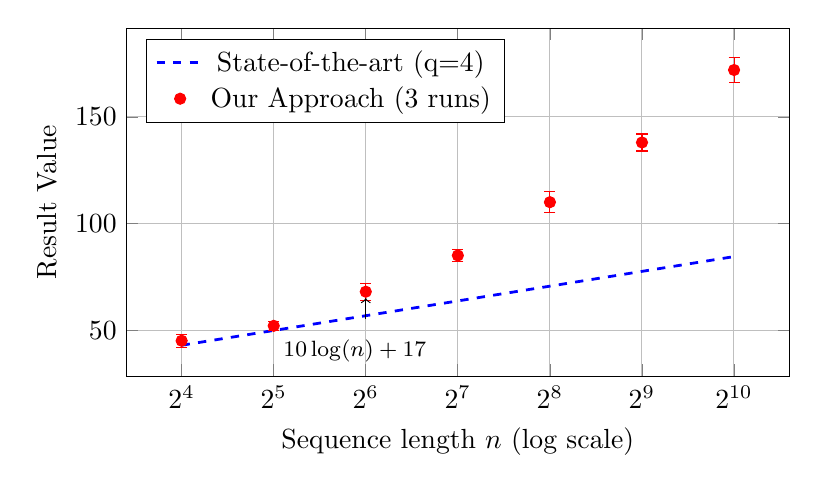
\begin{tikzpicture}
  \begin{axis}[
    xlabel={Sequence length $n$ (log scale)},
    ylabel={Result Value},
    xmode=log,
    log basis x={2},
    grid=both,
    legend pos=north west,
    width=10cm,
    height=6cm
  ]
  
  % State-of-the-art formula: 10log(n) + 3log(q) + 11 with q=4
  \addplot[
    domain=16:1024,
    samples=100,
    color=blue,
    line width=1pt,
    dashed
  ] {10*ln(x) + 3*ln(4) + 11}; % Using natural logarithm
  \addlegendentry{State-of-the-art (q=4)}
  
  % Our approach - simulated data points
  \addplot[
    only marks,
    color=red,
    mark=*,
    mark size=2pt,
    error bars/.cd,
    y dir=both,
    y explicit
  ] coordinates {
    (16, 45) +- (0, 3)
    (32, 52) +- (0, 2)
    (64, 68) +- (0, 4)
    (128, 85) +- (0, 3)
    (256, 110) +- (0, 5)
    (512, 138) +- (0, 4)
    (1024, 172) +- (0, 6)
  };
  \addlegendentry{Our Approach (3 runs)}
  
  % Annotations
  \node[anchor=west] at (axis cs:32,40) {\footnotesize $10\log(n) + 17$};
  \draw[->, thin] (axis cs:64,55) -- (axis cs:64,65);
  
  \end{axis}
\end{tikzpicture}
\end{document}